\section{Results}
\label{sec:results}

\subsection{Base-case life expectancy}
In the base-case analysis (age~40 at donation, overall population parameters), kidney donation was associated with a life-expectancy cost of $\Delta\text{LE} = -37.0$~days (donor 38.15~yr vs.\ non-donor 38.16~yr remaining life expectancy; analytic cohort). The Monte Carlo simulation ($5 \times 10^6$ individuals per arm) confirmed this estimate ($\Delta\text{LE} = -38.3$~days). Across all base-case and subgroup scenarios, donation was associated with a net life-expectancy cost to the donor; no scenario identified donation as neutral or beneficial to the individual.

\subsection{Racial disparity}
Race was the strongest subgroup modifier of life-expectancy cost (Figure~\ref{fig:age_race_sex_matrix}). Black donors experienced a cost of 73.4~days, nearly three times the 25.1~days estimated for White donors at age~40. The disparity widened sharply with younger age at donation: a Black donor at age~25 loses 199~days of life expectancy compared with 35~days for a White donor of the same age. This disparity traces directly to post-donation ESRD incidence: Black donors have a 15-year cumulative incidence of 74.7 per~10,000 versus 22.7 per~10,000 in White donors,~\cite{muzaale_risk_2014} a $3.3\times$ difference that is further compounded by a higher background ESRD rate in age- and health-matched Black non-donors.~\cite{grams_kidney-failure_2016}

\subsection{Age at donation}
The life-expectancy cost decreased monotonically with older age at donation, from 52.8~days at age~25 to 16.3~days at age~55 (Figure~\ref{fig:age_race_sex_matrix}). This gradient reflects the shorter remaining lifetime over which excess ESRD risk accumulates: younger donors have more life-years at risk and thus more opportunity for the elevated ESRD hazard to materialize.

\subsection{Sex}
Male donors faced a larger life-expectancy cost (43.6~days) than female donors (29.9~days), consistent with the male-sex within-donor ESRD hazard ratio of 1.88 reported by Massie et al.~\cite{massie_quantifying_2017} Sex and race effects compound: a Black male donor at age~40 loses 92~days, roughly double the 44~days for an overall male and six times the 14~days for a White female donor of the same age (Figure~\ref{fig:age_race_sex_matrix}). At age~25, Black male donors lose 249~days versus 29~days for White female donors.

\subsection{Probabilistic sensitivity analysis}
The PSA of 200~parameter draws (Figure~\ref{fig:psa}) produced a mean $\Delta\text{LE}$ of $+29.5$~days (95\%~credible interval $-1{,}085.5$ to $+1{,}068.0$~days; P[donation beneficial]~$= 48\%$). The wide credible interval and near-50\% probability of benefit are driven almost entirely by uncertainty in the donor all-cause mortality hazard ratio, which produces a tight cluster near $-37$~days when the HR is near its point estimate of 1.0 and a heavy left tail when the HR is drawn from the upper tail of the log-normal prior. Conditional on the HR remaining at 1.0, the value supported by the US-based literature and the O'Keeffe et al.\ meta-analysis,~\cite{okeeffe_mid-_2018} the model result is robustly and consistently negative.

\subsection{One-way sensitivity analysis}
\label{sec:owsa}
The donor all-cause mortality hazard ratio dominated all other parameters by an order of magnitude (Table~\ref{tab:owsa}, Figure~\ref{fig:tornado}). Setting HR~$= 1.30$~\cite{mjoeen_long-term_2014} increased the life-expectancy cost swing of more than 1,000~days from base case. No other parameter produced a swing exceeding 32~days. Dialysis mortality ($\pm 50\%$) shifted $\Delta$LE by at most $\pm 12$~days.

\subsection{Donor priority benefit}
Although KAS250 affords prior living donors (PLD) priority access to the deceased-donor waitlist,~\cite{wainright_impact_2017} the resultant life-expectancy benefit to the donor is negligible at the population level. Removing PLD priority access entirely, setting the donor waitlist to the standard 985-day median, worsened $\Delta$LE by only 1.9~days relative to base case. Halving the priority wait to 50~days recovered only 0.1~days. This insensitivity arises because fewer than 0.3\% of donors develop ESRD within 15~years and fewer still ever reach the transplant waitlist; the priority pathway is simply too rarely invoked to move a population-level outcome meaningfully.

\subsection{Voucher benefit}
The life-expectancy benefit of a kidney-donation voucher to a healthy, non-donor family member peaked at $+0.8$~days for a recipient designated at age~25, falling to $+0.3$~days at age~40 and $+0.1$~days at age~60. These small figures reflect the same dilution mechanism: conditional on developing ESRD and reaching the priority waitlist, priority access adds a clinically substantial $+605$~days of life expectancy for a patient whose ESRD onset occurs at age~40, and $+209$~days for onset at age~60 (Figure~\ref{fig:esrd_conditional}). However, since only approximately 0.04\% of non-donors develop ESRD within 15~years, this large conditional benefit compresses to well under one day at the population level. Voucher benefit was modestly higher for Black non-donor family members ($+1.7$~days at age~40), owing to their approximately four-fold higher baseline ESRD incidence.~\cite{grams_kidney-failure_2016}

% \begin{figure}[t]
%   \centering
%   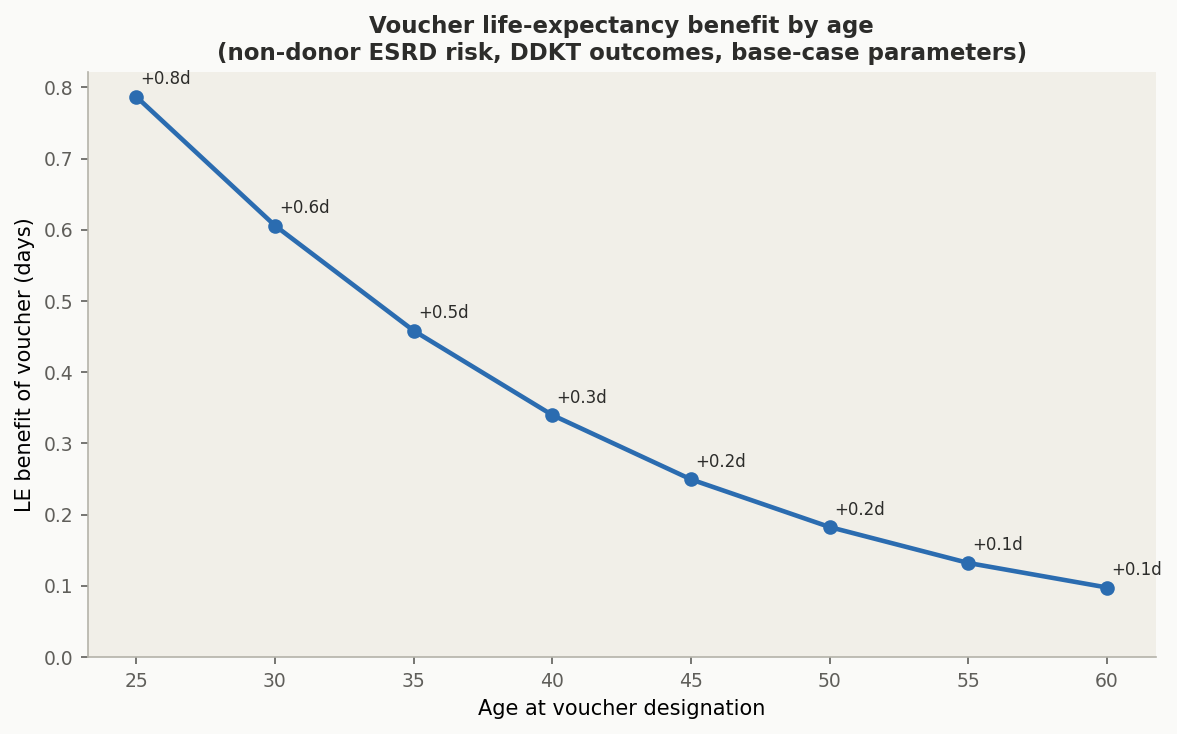
\includegraphics[width=\linewidth]{figures/voucher_cohort_age_sweep.png}
%   \caption{\textbf{Voucher life-expectancy benefit by age at designation.} $\Delta$LE (voucher holder minus unvouched non-donor, days) for a healthy non-donor family member carrying a kidney-donation voucher, as a function of the age at which the voucher is designated. Both arms carry non-donor ESRD risk. The benefit declines with age because older individuals have less remaining lifetime over which the voucher's priority access could be exercised. Even at the maximum (age~25, $+0.8$~days), the benefit is small at the population level due to the low baseline ESRD incidence among non-donors.}
%   \label{fig:voucher}
% \end{figure}